\section{Tarefas no Âmbito do Projeto RIL}\label{sec:def_e_inc}

    Devido à natureza rotativa da equipa, foram efetuadas várias tarefas no âmbito do projeto. Nesta secção vamos analisar alguns dos testes, \textit{defects}, incidentes bem como outras tarefas que tenham sido concretizadas no contexto do estágio académico. Devido ao vasto número de incidentes e defeitos explorados e à natureza efémera da análise destes, visto que frequentemente a análise seria transferida para outra pessoa e ao curto tempo de análise, foi escolhida uma abordagem onde se vai analisar a fundo apenas algumas das tarefas, de forma a se detalhar bastante o processo.

    A participação do presente estagiário no projeto inicia-se em simultâneo um com colega, que já colaborava com a Deloitte, mas que era estranho ao projeto. Assim aproveitou-se para ambos aprenderem acerca das ferramentas e da lógica juntos em todas as circunstâncias em que tal fazia sentido.

    Como procedimento de acolhimento a recém-chegados, há uma fase inicial, após as formações iniciais mencionadas na Secção \ref{formacoes_introdutorias_empresa_cliente}, onde novos membros acompanhavam outros membros da equipa nas suas tarefas, como, por exemplo, as tarefas que acompanhavam dependiam das tarefas que estariam a ser realizadas na altura. Com tempo, passariam a fazer estas tarefas individualmente.

        \subsection{Resolver \textit{Defects}}\label{sub:defects}

        Nesta secção vão-se explorar a fundo alguns dos \textit{defects} resolvidos durante o período do estágio, incluindo ferramentas e métodos de trabalho e análise utilizados. Este método foi escolhido de forma a que o leitor possa ficar com uma ideia clara do que é necessário e importante no processo do trabalho atribuído, desta forma uma análise profunda pode ser executada evitando uma análise mais supreficial de todas. Para uma visão holística do trabalho, a Tabela \ref{defeitos_trabalhados} detalha todos os \textit{defects} trabalhados, respetivas prioridades.
        
        \begin{table}[htbp] % htbp
            \centering
            \caption{\textit{Defects} Trabalhados}
            \label{defeitos_trabalhados}
            \source{Documentação Interna} % 1- https://impalaintech.com/blog/mendix-vs-outsystems-vs-appian/
            \begin{tblr}{
                % example for tblr: https://tex.stackexchange.com/questions/603349/tabularray-and-new-command-for-multicolumn-cells
                % another example: https://tex.stackexchange.com/questions/605676/tabularray-how-to-control-the-vertical-alignment-of-the-cells-contents
                hlines={lightgray}, vlines={lightgray},
                width = \linewidth,% total width set to width available
                %rows = {c,m}, % c aligns horizontally, m aligns vertically, aligns all rows
                colspec={X[3,c,m] X[3.5,c,m] X[c,m] X[c,m] X[1.2,c,m]},
            }
            % \textbf{Tempo trabalhado}
            \textbf{Título do \textit{defect}} & \textbf{Descrição do \textit{defect}} & \textbf{Prioridade} \\

            % Low, Medium, High, Critical

            ``A Withdrawn FO showing 'Requested' in overview screen \& 'Invalid Data' error message appearing when clicked on 'Requested''' & Um \textit{broker}, ao receber um FO, e esta ser retirada de seguida, o \textit{broker} consegue visualizar ``requested'' na tab ``overview'' para alguns dos UWs. Quando o \textit{broker} clica no estado ``requested'', surge uma mensagem de erro ``Invalid Data''. & Baixa \\

            ``The broker can't find the contract using the filter despite the UMR contract is showing in the filter that exists.'' & Contratos não conseguiam ser encontrados através dos filtros de procura. & Média \\

            ``Regression - Subjectivity email notifications - Wrong emails getting triggered for subjectivity flow'' & Quando o UW apaga uma \textit{subjectivity} com o estado de ``satisfaction pending'', a subjetividade passa para o estado ``Proposed Deletion''. E quando o Broker aceita a proposta de exclusão da \textit{subjectivity}, o e-mail/notificação ``Firm Order - Update'' é acionado em vez do e-mail/notificação ``Subjectivity Deleted''. & Média \\

            ``Amend Master Facility - UW not visible at Overview tab and Sign and Close page'' & O UW não se encontra visível na tab \textit{Overview} quando se efetua uma alteração à MF. & Média \\

            ``PRE - Master Facility - Post Bind Reference or Risk code changes are not showing any stamp details in the transaction logs'' & Ao criar um novo contrato, em certas situações, detalhes dos \textit{stamps} não eram criados. Não foi possível reproduzir. & Média \\

            ``Stamp Visibility | Broker - The UW stamps should be filtered by the company.'' & Refira à Secção \ref{visibilidade_de_stamp_defect} & Média \\

            ``Index out of bounds when submiting cancel and replace'' & Refira à Secção \ref{index_out_of_bounds_defect} & Urgente \\
            \end{tblr}
        \end{table}

        Vamos, primeiramente, detalhar a forma de análise de \textit{defects}:

        \subsubsection{Análise de \textit{Defects}}\label{secsec:analise_de_defects}

            De uma forma geral, os passos na análise e resolução de um \textit{defect} devem seguir os seguintes pontos:

            \begin{enumerate}
                \item A análise começa pela reflexão sobre se o \textit{defect} está contemplado, ou não, nas USs, ou seja, se não será um GAP;
                
                Sendo um GAP, é passado à equipa relevante para a US ser alterada, caso contrário avança-se para o próximo passo: 
                \item De seguida deve-se identificar o ambiente em que se deve testar e resolver o \textit{defect};
                
                Existe um campo ``Target Fix Release'' que indica a release em que o \textit{defect} deverá ser resolvido, esta informação deve ser ligada ao \textit{deployment aggregator} para identificar em qual dos ambientes de desenvolvimento se deve prosseguir, no caso dos ambientes do protótipo da Figura \ref{fig:deployment-aggregator}, os ambientes DED ou DES.  
                \item Deve-se então atualizar o ``Assignee'' para o nosso utilizador na plataforma;
                \item Analisar, preparar e corrigir o \textit{defect} na plataforma Service Studio atualizando sempre o estado no \textit{defect} apropriadamente, neste caso de \textit{New} para \textit{In Analysis} para \textit{Ready For Development} conforme o flow demonstrado na Figura \ref{fig:defect-workflow};
                \item De seguida o mais apropriado será alinhar com os maestros. Para tal será necessário realizar testes e revisões do código e possivelmente retrofit para um ambiente mais a baixo, são também criadas ``subtasks'' para estas tarefas que são, no entanto,  frequentemente realizadas por outras equipas. 
            \end{enumerate}

        \subsubsection{Índice fora dos limites ao submeter \textit{Cancel and Replace}}\label{index_out_of_bounds_defect}

        \textit{Defect} original: ``\textit{Index out of bounds when submiting cancel and replace}''

            % ``defect com a liliana'' no onenote

            Um dos primeiros \textit{defects} analisados, foi analisado em conjunto com um membro da equipa numa dinâmica de \textit{Remote Pair Programming}.

            \textbf{\textit{Pair Programming}}: Também conhecido por \textit{peer programming}, é um estilo de programação ágil onde dois programadores trabalham em conjunto no mesmo dispositivo e no mesmo problema\cite{peer-programming}. Existe debate àcerca do método e da sua eficácia, mas tem sido observado, sendo benéfico, em casos em que a tarefa é complexa e uma alta precisão no código é essencial, bem como em tarefas simples onde o tempo é limitado. É também uma boa forma de aprendizagem e integração, onde participantes reportam resultados positivos em áreas como a aprendizagem, confiança no código, tempo necessário e gosto geral no processo\cite{faja2014evaluating,hannay2009effectiveness}. % \parencites{faja2014evaluating}{hannay2009effectiveness}. 

            \begin{table}[htbp] % 
                \centering
                \caption{Detalhes do defeito '\textit{Index out of bounds when submitting cancel and replace}'}\label{table:defect1}
                \source{Documentação Interna}
                \begin{tabularx}{1\textwidth}{|>{\raggedright\arraybackslash}X|}
                    \hline
                    \rowcolor{lightgray}
                    \textbf{\textit{Defect}} \\
                    \hline
                    \rowcolor{lightgray!20}
                  
                    \begin{quote}
                        \textbf{Descrição do Defeito:}

                        Ao fazer uma correção do tipo \textit{Cancel and Replace}, quando o \textit{broker} submetia a correção ao \textit{underwriter}, aparecia o erro: ``Index out of bounds. Index -1 for bounds [0,0]''.
                        
                        \begin{itemize}
                            \item Resultado Atual: Ocorre o erro: ``Index out of bounds. Index -1 for bounds [0,0]'';

                            \item Resultado Esperado: O \textit{broker} deve ser capaz de enviar a correção ao \textit{underwriter} sem erros;

                            \item Possível Continuar com o Fluxo: Não;

                            \item Solução Alternativa: Não há;

                            \item Passos para Reproduzir:
                            \begin{itemize}
                                \item Criar um \textit{placement} com 1 \textit{underwriter};

                                \item Enviar um pedido de Firm Order;

                                \item Aceitar o pedido de Firm Order;

                                \item O \textit{broker} cria uma correção do tipo \textit{Cancel and Replace};

                                \item Não fazer alterações pelo \textit{Cancel and Replace};

                                \item Submeter o pedido pressionando ``Send Correction to Underwriter'';

                                \item Ao seguir estes passos, o erro ``Índice fora dos limites. Índice -1 para limites [0, 0]'' deve ser exibido.
                            \end{itemize}
                        \end{itemize}
                    \end{quote}

                    \\
                    \hline
                \end{tabularx}
              \end{table}

            \subsubsubsection*{Análise e Resolução:}

                A descrição do \textit{defect} em causa encontra-se na Tabela \ref{table:defect1}. Fazendo a análise segundo a Secção \ref{secsec:analise_de_defects}:

                \begin{enumerate}
                    \item Neste caso, visto que o \textit{defect} se referia a um erro de limites que aparecia na própria plataforma, não foi necessário procurar a US referente à funcionalidade, isto porque facilmente se deduz ser um comportamento causado por um erro no código que não é desejado na lógica de negócio;

                    \item Nesta etapa foram feitos testes que demonstraram que o erro se encontrava apenas num dos ambientes de desenvolvimento, pelo que se procedeu a analisar e resolver o defeito neste ambiente;

                    \item Já se tinha atualizado o ``Assignee'';

                    \item A fase de análise e correção é sempre a mais demorada e imprevisível, sempre atualizando o estado do \textit{defect} quando apropriado:
                    
                    O processo de desenvolvimento e resolução está muito dependente da comunicação com os membros mais adequados da equipa para cada etapa, pelo que grande parte da capacidade de resolução de problemas, especialmente numa fase inicial, depende muito de uma capacidade de comunicação com os colegas de trabalho. 

                    A análise começou com uma troca de informação com uma BA familiarizada com o flow de \textit{cancel and replace} que nos direcionou para a ação com a lista onde provavelmente ocorria o problema.

                    De seguida fomos à ação em causa, ativamos o debugger do Service Studio, fizemos um \textit{cancel and replace} na plataforma e identificamos a causa do problema, como é possível ver na Figura \ref{fig:index_out_of_bounds1}, o ID do contrato chegava vazio à lista. 

                    \begin{figure}[H]
                        \centering
                        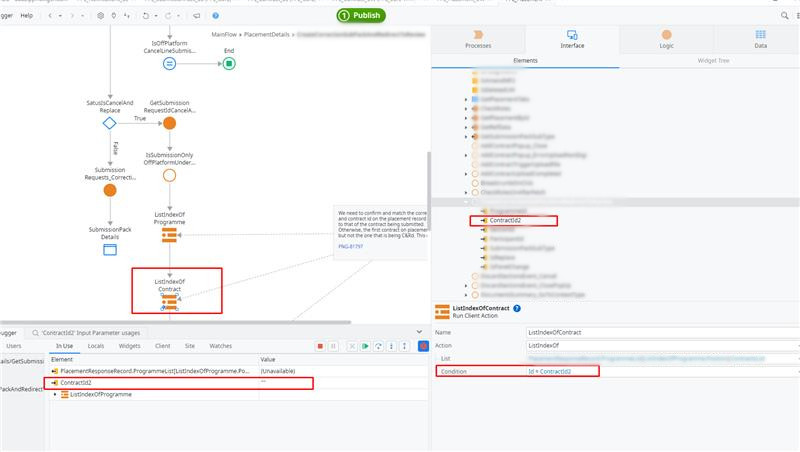
\includegraphics[width=\textwidth]{imgs/IndexOutOfBounds1.jpg}
                        \caption{Index Out of Bounds - Root of the Problem}\label{fig:index_out_of_bounds1}
                        \source{Service Studio Interno}
                    \end{figure}

                    Analisou-se então a interface e de onde vinha o ID do contrato inicialmente ao pressionar o botão, e descobriu-se que o ID era passado ao bloco corretamente. Portanto, era no meio da comunicação, desde quando se clicava no botão até à ação em questão, que se perdia o valor.

                    Os dados eram passados quase exclusivamente de blocos para blocos a partir de \textit{block events}.

                    \textbf{Blocos em OutSystems}: É uma interface reutilizável com código, widgets, ou outros blocos \cite{os-blocks}.

                    \textbf{Eventos de Blocos}: São eventos que permitem ao bloco interagir com o parente do bloco. Estes eventos podem ter variáveis de input ou de output, visto que o ecrã ou o bloco pai não sabe se algo acontece no bloco, como um botão ser clicado, usam-se eventos para passar esta informação para fora, que podem também ser de caráter obrigatório\cite{os-block-events}.

                    Havia uma passagem da informação entre 4 blocos, cujos eventos chamavam diretamente outros eventos, sem haver oportunidade de colocar \textit{breakpoints} no meio do fluxo, depois de uma troca entre um colega acerca do funcionamento de \textit{triggers} em OutSystems, procedeu-se à criação de ações auxiliares que apenas chamavam eventos, e fez-se com que os eventos chamassem estas ações. Desta forma já era possível colocar \textit{breakpoints} e descobrir em que passagem se perdiam os dados. 
                    
                    Veio-se a descobrir que na passagem onde se perdiam os dados, o nome da variável de onde vinham os dados de um bloco era igual ao nome da variável para onde iam os dados noutro bloco, isto normalmente não seria um problema, mas, OS, com o seu código interno em C\#, tem dificuldades em fazer um registo e passagem correta de dados em caso de nomes iguais, pelo que se procedeu à mudança do nome e à publicação da aplicação, o que acabou por solucionar o problema.
                    
                    Retiraram-se então as ações auxiliares e atualizou-se o estado do \textit{defect} adequadamente;
                    
                    \item Nesta etapa comunicou-se com o nosso líder de equipa, e foi necessário reverter as mudanças. O leitor pode-se ter apercebido que o segundo ponto não seguia o padrão de análise de \textit{defects} estabelecido na Secção \ref{secsec:analise_de_defects}. Era necessário analisar o \textit{deployment aggregator} e não apenas resolver o defeito no ambiente de desenvolvimento em que este ocorria. 
                    
                    Veio-se a descobrir que durante aquele período o código de ambas as plataformas de desenvolvimento deveria ser idêntico dado que o código de uma iria substituir a outra brevemente. Pelo que a resolução foi revertida e a análise foi guardada apenas como informação no \textit{defect}, que mais tarde foi usada por um colega que aplicou a resolução na altura e no ambiente correto.
                \end{enumerate}

        \subsubsection{Visibilidade de stamp | Corretora — Os stamps de UW devem ser filtrados pela empresa}\label{visibilidade_de_stamp_defect}

        \textit{Defect} original: ``\textit{Stamp Visibility | Broker - The UW stamps should be filtered by the company}''

            \begin{table}[htbp] % htbp
                \centering
                \caption{Detalhes do defeito '\textit{Stamp Visibility | Broker - The UW stamps should be filtered by the company}'}\label{table:defect2}
                \source{Documentação Interna}
                \begin{tabularx}{1\textwidth}{|>{\raggedright\arraybackslash}X|}
                    \hline
                    \rowcolor{lightgray}
                    \textbf{\textit{Defect}} \\
                    \hline
                    \rowcolor{lightgray!20}
                  
                    \begin{quote}
                        \textbf{Descrição do Defeito:}
                    
                        Um \textit{broker} cria um novo contrato, depois de preencher todas as informações obrigatórias e carregar o documento MRC (documento obrigatório para contratos), seleciona um UW que participará no contrato.
    
                        Se selecionar um UW A (Empresa X), que pertence a várias equipas dentro da Empresa X e Empresa Y (ambas as empresas estão sob a mesma organização), quando seleciona ``Permitted Territory'' - ``Show All'', só devo ver todos os stamps que o UW A tem atribuídos na Empresa X, mas vê-se os stamps atribuídos na Empresa X e Y.
    
                        \begin{itemize}
                            \item Passos para Reproduzir:
                                \begin{itemize}
                                    \item Criar um contrato;
                                    \item Selecionar um UW que pertence a 2 ou mais empresas da mesma organização;
                                    \item Selecionar ``Show All'' no território permitido;
                                    \item Validar se os stamps disponíveis para o \textit{broker} são os stamps atribuídos ao UW dentro dessa empresa.
                                \end{itemize}
                        \end{itemize}
                    \end{quote}

                    \\
                    \hline
                \end{tabularx}
            \end{table}
            
            \subsubsubsection*{Análise e Resolução:}

                A descrição do \textit{defect} encontra-se na Tabela \ref{table:defect2}. Começou-se a análise pela verificação da US associada à funcionalidade, depois de uma troca com um membro da equipa familiarizado com as USs, identificou-se a US da Tabela \ref{table:us1}.

                \begin{table}[H] % htbp
                    \centering
                    \caption{Detalhes da US ``\textit{List of Stamps - Add a Stamp}''}\label{table:us1}
                    \source{Documentação Interna}
                    \begin{tabularx}{1\textwidth}{|>{\raggedright\arraybackslash}X|}
                        \hline
                        \rowcolor{lightgray}
                        \textbf{User Story:} Lista de stamps --- Adicionar um stamp \\
                        \hline
                        \rowcolor{lightgray!20}
                      
                        \begin{quote}
                            \textbf{Visão da User Story:} Para a configuração de um Transportador, os stamps estão vinculados à hierarquia (Organização, Empresa e Utilizador). Esta US permitirá a criação de uma lista de stamps. A lista de stamps também incluirá a ocultação de stamps inativos na lista global.
                        
                            \textbf{Como...} Administrador RIL
                        
                            \textbf{Eu quero...} Adicionar um stamp
                        
                            \textbf{Para quê...} Configurar uma lista de stamps
                        
                            \textbf{Critérios de Aceitação de Negócios:}
                        
                            \textbf{Configuração inicial do ecrã de stamps:}

                            \begin{itemize}
                                \item Dado o Administrador RIL estar no ecrã ``hierarquia'' \newline
                                Quando o Administrador RIL seleciona a aba ``stamps'' \newline
                                Então, a descrição da aba será ``lista de stamps'';

                                \item Dado o Administrador RIL estar na tela ``hierarquia'' \newline
                                Quando o Administrador RIL seleciona a aba ``stamps'' \newline
                                Então, mostra as seguintes colunas de dados (na ordem listada): Nome do stamp, tipo de agência, tipo de stamp, válido a partir de, válido até, estado, classificação e ação;

                                \item Dado o Administrador RIL estar no ecrã ``hierarquia'' \newline
                                Quando o Administrador RIL seleciona a aba ``stamps'' \newline
                                Então, por defeito, mostrar uma lista de carimbos ATIVOS para a organização;
                            
                                \item \textit{etc.}
                            \end{itemize}
                            
                        \end{quote}
                        \\
                        \hline
                    \end{tabularx}
                \end{table}

                Após a análise desta US, deduziu-se que se tratava de um GAP, isto porque na US original dizia ``por defeito, mostrar uma lista de carimbos ATIVOS para a organização'', não implicando que devam ser filtrados por empresa. Esta filtragem não se faz na aplicação, e isso torna-se evidente neste caso em que o utilizador pertence a várias equipas de diferentes empresas da mesma organização.

                Foi então reportado no próprio \textit{defect} e notificadas as equipas relevantes, que continuaram com o problema a partir daí.

            % Outro defect Defect [PNG-74147] Stamp Visibility | Broker - The UW stamps should be filtered by the company. - Jira (atlassian.net)

        \subsection{Reportar \textit{Defects}}\label{sub:reportar_defects}

        Pode acontecer que através de testes, ou incidentes, ou mesmo apenas usando a plataforma, se depare com um erro ou comportamento inesperado, o qual pode ter que ser reportado como defeito. Circunstância esta que aconteceu ao presente estagiário quando conseguiu carregar dois documentos MRC para apenas um contrato, algo que não devia ser possível. 

        Ocorria também, com alguma frequência, membros da equipa descobrirem defeitos durante o apoio a testes. Como parte do seu trabalho cabia-lhes, mediante solicitação,  
        ajudar a documentá-los e a registá-los na plataforma Jira. Na Tabela \ref{tab:table_reported_defects} encontram-se listados todos os defeitos reportados durante percurso do estágio.

        O processo de reportar defeitos é bastante intuitivo e envolve a criação de uma entrada no Jira, onde são fornecidos detalhes essenciais para a compreensão e resolução do problema. Este processo implica frequentemente a confirmação com membros da equipa sobre campos cruciais, como a versão principal, tipo de defeito, data de deteção, fase de teste, \textit{sprint}, versão afetada, severidade e prioridade.

        Detalhes adicionais, como descrição, passos para reproduzir o defeito, se o utilizador fica ou não bloqueado, qual a solução alternativa, resultado esperado e resultado atual, são também incluídos no registo do defeito. Este nível de detalhe facilita a triagem, análise e resolução eficaz por parte da equipa de desenvolvimento futuramente.

        \begin{table}[htbp] % htbp
            \centering
            \begin{tblr}{
                % example for tblr: https://tex.stackexchange.com/questions/603349/tabularray-and-new-command-for-multicolumn-cells
                % another example: https://tex.stackexchange.com/questions/605676/tabularray-how-to-control-the-vertical-alignment-of-the-cells-contents
                hlines={lightgray}, vlines={lightgray},
                width = \linewidth,% total width set to width available
                %rows = {c,m}, % c aligns horizontally, m aligns vertically, aligns all rows
                colspec={X[3,c,m] X[3,c,m] X[1,c,m] X[1,c,m]},
            }
            % \textbf{Tempo trabalhado}
            \textbf{Título do \textit{defect}} & \textbf{\textit{Defect} em Português} & \textbf{Assigned by the end of the internship} & \textbf{Repórter} \\

            PNG-89894 Copy Panel Button Appears for a moment in the wrong context & Botão \textit{Copy Panel} Aparece por um Momento no Contexto Errado & Assigned & João Filipe Silva de Almeida \\
            PNG-88375 Unable to Replace Contract Endorsement document & Não é Possível Substituir o Documento do \textit{Endorsement} do Contrato & Unassigned & João Filipe Silva de Almeida \\
            PNG-88371 INC0067421, INC0067542 --- Adding multiple contract documents to a contract & Possível Adicionar vários Documentos a um Contrato & Assigned & João Filipe Silva de Almeida \\
            PNG-88069 INC0065686-UW able to accept withdrawn request & UW Capaz de Aceitar Pedidos \textit{Withdrawn} & Unassigned & João Filipe Silva de Almeida \\
            PNG-87070 PROD --- "Mark as backloaded" option in contracts shouldn't appear in Archived Placements. & Opção "Mark as backloaded" em Contratos não Deve Aparecer nas Colocações Arquivadas & Assigned & João Filipe Silva de Almeida \\
            PNG-87058 INC0063053, INC0065981 --- Endorsement showing "not Responded" & \textit{Endorsement} Mostrando "Não Respondido" & Unassigned & João Filipe Silva de Almeida \\
            PNG-83536 INC0062203, INC0067349, INC0068073, INC0069140, INC0071112 --- UW Reference changes by UW aren't inherited by contract endorsements & Alterações nas Referência feitas por um UW não são Herdadas por \textit{Endorsements} do Contratos & Assigned & João Filipe Silva de Almeida \\
            PNG-83098 INC0064504 --- Regression(Prod) --- status withdraw blinks in overview tab in broker & Regressão (Produção) --- \textit{Withdrawn} Status Pisca na aba \textit{Overview} com o \textit{Broker} & Assigned & João Filipe Silva de Almeida \\

            \end{tblr}
            \caption{Defeitos Reportados}
            \label{tab:table_reported_defects}
            \source{Documentação Interna} % 1- https://impalaintech.com/blog/mendix-vs-outsystems-vs-appian/
        \end{table}

        % tipo o de adicionar vários contratos a um documento: 

        % Podes filtrar no Jira por reported by me

        \subsection{Análise de Incidentes}\label{sub:incidentes}

        Incidentes, ao contrário de \textit{defects}, têm uma certa urgência associada, devido a serem um problema reportado diretamente por um utilizador, havendo, normalmente, alguém à espera que este seja resolvido. Pelo que se recorre muito mais a \textit{datafixes} para desbloquear utilizadores e nem sempre é possível ou viável chegar à causa, ou raiz dos problemas.

        % ``O meu primeiro Incident'' No onenote INC0063053

        \subsubsection{INC0064225 - Todas as seleções são inválidas}\label{secsec:inc0064225} % INC0064225 com o marcio

            Incidente original: ``\textit{All selections invalid}''

            % OMG INCIDENTE INC0064225, aquele que fizeste datafix com o marcio

            \begin{table}[H] % htbp
                \centering
                \begin{tabularx}{1\textwidth}{|>{\raggedright\arraybackslash}X|}
                    \hline
                    \rowcolor{lightgray}
                    \textbf{Incidente INC0064225} \\
                    \hline
                    \rowcolor{lightgray!20}
                
                    \textbf{Descrição do Incidente:} O utilizador ficou bloqueado ao submeter uma nova Firm Order. Depois de fazer o processo todo de submissão como esperado, aparecia o erro ``All selections are invalid, Please review the breakdown below and select Cancel to return to the Submission Pack'', apresentando por baixo uma lista com todos os UWs a dizer estarem inativos.

                    \\
                    \hline
                \end{tabularx}
                \caption{Incidente INC0064225}\label{table:usincINC0064225}
                \source{Resumo da Informação do Incidente no Service Now}
            \end{table}

            A descrição do incidente encontra-se na Tabela \ref{table:usincINC0064225}.

            Durante a investigação, verificou-se um possível equívoco no número fornecido pelo utilizador ``NM0011234'', que se presumiu que deveria ser ``NM0011224''. 

            Identificou-se inicialmente a possibilidade de resolver o problema removendo e adicionando novamente a \textit{Master Facility} à declaração. Esta abordagem foi sugerida ao utilizador, como uma solução potencial para o problema.
            
            Ao analisar as participações associadas à \textit{Facility}, notou-se ainda uma discrepância numa delas, relacionada com um utilizador chamado ``John''. Embora não pareça ser a causa direta do problema, esta discrepância foi registada para investigação adicional, caso a solução inicial não fosse bem-sucedida.

            Foi então mandado o pedido ao utilizador para adicionar a MF de novo. Recebeu-se resposta negativa atempadamente, informando-nos que isto já fora tentado e não funcionara.
            
            No entanto, na base de dados era possível ver que a última mudança ao contrato fora há mais de uma semana atrás, foi decidido, portanto, fazer a \textit{datafix} para corrigir o utilizador ``John'' e marcar uma reunião com o utilizador. Devido ao tempo que o \textit{datafix} levou a ser aplicado, acabou por não se conseguir falar com o utilizador antes do final da semana. Mas mais tarde recebeu-se a notícia que o \textit{datafix} efetuado fora suficiente para desbloquear o utilizador e o incidente pôde ser fechado.
            
        \subsubsection{INC0065686 - Não foi possível enviar o cancelamento}\label{secsec:inc0065686} % INC0064225 com a ines
                
            Incidente original: ``\textit{Unable to submit cancelation}''

            \begin{table}[H] % htbp
                \centering
                \begin{tabularx}{1\textwidth}{|>{\raggedright\arraybackslash}X|}
                    \hline
                    \rowcolor{lightgray}
                    \textbf{Incidente INC0065686} \\
                    \hline
                    \rowcolor{lightgray!20}
                
                    \textbf{Descrição do Incidente:} O utilizador mandou uma Firm Order para um UW que não devia ter mandado, por isso clicou em ``withdraw'' do pedido, mas o UW conseguiu aceitar. Ao ver que o UW tinha aceite, foi mandado um pedido de cancelamento, mas o UW não conseguia visualizá-lo, e ao abrir a submissão deste pedido, o programa fica parado a carregar infinitamente.

                    \\
                    \hline
                \end{tabularx}
                \caption{Incidente INC0065686}\label{table:incINC0065686}
                \source{Resumo da Informação do Incidente no Service Now}
            \end{table}

            A descrição do incidente encontra-se na Tabela \ref{table:incINC0065686}.

            No decorrer da análise do incidente INC0065686, foi identificado o problema na base de dados. Existe uma sequência de documentos criados na DB de MongoDB que são criados quando o estado de um UW é mudado, estas são as negotiations. Depois de se comunicar com um membro da equipa familiarizado com o funcionamento desta coleção, apercebeu-se que depois da negotiation com o estado ``withdrawn'' foi gerada subsequentemente uma negotiation com o estado \texttt{pending\_unconditional\_line}, que significa que o pedido tinha sido enviado para o UW mesmo tendo sido withdrawn; se fosse um novo pedido e não o mesmo, teria que haver uma negotiation \texttt{request\_for\_line\_or\_binder} antes da \texttt{pending\_unconditional\_line}.

            Não foi encontrada nenhuma indicação na Base de Dados do pedido de cancelamento descrito pelo utilizador.

            Depois de alguma discussão decidiu-se que a solução seria fazer um ``soft delete'' das negociations depois do withdraw. Para manter a integridade da base de dados foi necessário também alterar a coleção das ``participations'', que continha informação àcerca do UW e da sua participação atual no contrato, tendo sido necessário remover cinco campos que tinham sido inadvertidamente adicionados devido às negotiations erróneas que foram criadas, e alterado o campo status da participation para ``new''.
            
            No fim foi criado um \textit{defect} com os passos para reproduzir que estavam por definir, onde se detalhou o problema: ``UW capaz de aceitar pedido withdrawn''.

            % INC INC0065686 (aquele que viste com a inês e foi preciso mandar datafix para remover as negotiations)

            % Incidente do Craveiro no onenote
            %  aquele que falaste com o user com a andereia, e que o problema era os subpanels

        \subsection{Testes}\label{sub:tests}

        Durante o período de estágio, as responsabilidades incluíam a realização de testes sempre que solicitado pela equipa. O processo de teste envolvia uma abordagem sistemática para garantir o funcionameninto e integridade adequados das funcionalidades desenvolvidas, e pode-se dividir nos seguintes passos:

        \begin{itemize}
            \item \textbf{Recebimento das Solicitações de Teste:} Ao ser solicitado, forma-se uma compreensão dos requisitos e casos a testar. Como por exemplo a identificação do ambiente a testar, e recolha de quaisquer documentos que possam ser necessários;
            \item \textbf{Recriação das condições do Teste:} Criação das condições na plataforma para recriar o teste com base nas especificações fornecidas;
            \item \textbf{Execução de Testes:} Interação com a aplicação, seguindo as especificações do teste, recolhendo evidências videográficas se necessário;
            \item \textbf{Registo de Resultados:} Documentação dos resultados, por exemplo, no defeito em causa, incluindo comportamentos inesperados e evidências;
            \item \textbf{Comunicação com a Equipa:} Segue-se o relato conciso dos resultados obtidos com quem os solicitou.
        \end{itemize}

        A principal destreza necessária para realizar estes testes é uma boa perceção da lógica de negócio e da plataforma. Os seguintes são alguns exemplos de testes feitos durante a duração do estágio:

        \begin{itemize}
            % Um da bárbara sobre a proposed line não ser revertida
            \item Criação de um contrato com duas secções, ambas com uma mistura de UWs off e on platform e uma mistura de \textit{roles} entre eles, mandar e aceitar o contrato, fazer uma \textit{correction} do tipo ``panel change'' e alterar a percentagem proposta por cada UW sem \textit{roles} de 60\% para 50\%. Aceitá-las na \textit{section} 1 e rejeitá-las na \textit{section} 2. Na \textit{section} rejeitada, deveria voltar a 50\% | 50\% proposed, em vez de 50\% | 60\%. O comportamento esperado foi o observado pelo que não se replicou;
            % Outro da Bárbara(e agora que tens que ver o codigo) sobre os archive placements
            \item Carregar \textit{placements} arquivados a partir de uma folha Excel onde o \textit{placing broker} especificado pertencia a uma organização com duas companhias diferentes onde ambas tinham \textit{branches} com nomes idênticos. Isto fazia com que ao ir buscar o utilizador do Excel, este pudesse ser extraído do \textit{branch} errado, resultando no bloqueio do utilizador devido à plataforma considerar estes dados inválidos;
            % Um teste sobre Receber notificações: on cancelation
            \item Criar uma \textit{declaration} com um \textit{leader} e um \textit{follower}, nenhum dos UWs têm \textit{roles}, enviar e aceitar, selecionar ``cancel line'' na declaration e enviar. Notar que o \textit{follower} não recebeu notificação da \textit{cancelation};
            % Podes falar dos testes que a Inês te deu, por exemplo o dos endorsements
            \item O preenchimento de uma folha de Excel acerca da informação presente no documento gerado pelos contratos e \textit{endorsements} dos contratos numa variedade de casos diferentes com UWs off e on platform.
        \end{itemize}

        \subsection{Análise de Processos}\label{sub:processos}

        Uma das tarefas delegadas ao presente estagiário foi também a análise de processos de OS. Dentro do Service center é possível analisar nas abas ``Monitoring'' e ``Processes'' os processos da aplicação e como é que estes foram concluídos ou em que estado estão, na Figura \ref{fig:interface_processo_servicecenter} pode-se ver a interface da plataforma ao visualizar os detalhes de um processo.

        Os processos aqui analisados são processos que acabavam suspensos, muitas vezes bastante antigos. São processos que causariam problemas a utilizadores se estes interagissem com o contrato específico associado a este processo, frequentemente podiam ser recomeçados e continuariam normalmente, mas em muitas das situações isto não acontece, esta situação oferece a possibilidade de identificar problemas com a plataforma e possíveis erros a resolver.

        \begin{figure}[H]
            \centering
            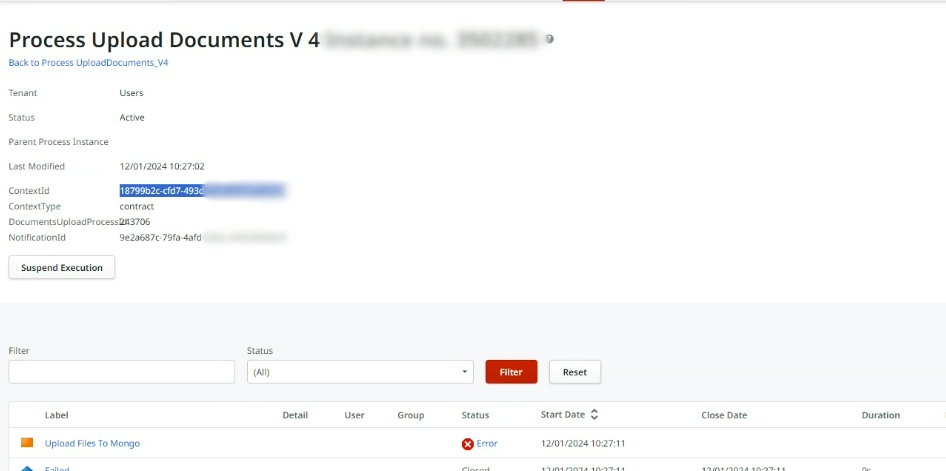
\includegraphics[width=\textwidth]{imgs/ProcessoServiceCenter.png}
            \caption{Interface de análise de um processo - Service Center}\label{fig:interface_processo_servicecenter}
            \source{Service Center Interno}
        \end{figure}

        Todos os processos revistos, independentemente do seu estado, tinham que ser anotados num documento de Excel específico para a tarefa com informação dos IDs dos contratos, \textit{placements}, equipas e utilizadores associados ao processo, bem como os erros ocorridos, caso tal seja relevante.

        Devido à natureza frequentemente repetitiva da análise destes, foi elaborado um web scraper em python que auxiliou na análise de alguns processos, por exemplo, foi automatizado o caso em que o processo \texttt{GenerateMRCEmailProcess} estava associado a um utilizador que estivesse inativo, registando e clicando ``skip'' na plataforma automaticamente, para mais informações refira à Secção \ref{secsec:scriptspython}.

        Existem três tipos de processos que geravam erros e era preciso analisar:

        \subsubsection{\texttt{SDC\_Generation}}\label{secsec:sdc_generation}

            % Isto é por causa da equipa de SDC para não sobrecarregarem

            Possivelmente o mais difícil de se analisar dos processos aqui representados.

            Foi imposto um limite de dez processos por hora e cinquenta por dia dos recomeçados com sucesso, de forma a não sobrecarregar a equipa dos processos.

            OS erros levantados neles tinham origem nos stamps das negociações e das suas complexidades. Devido à sua natureza volátil, e a criarem \textit{roles} diferentes para utilizadores e terem uma lógica de pertença a utilizadores e organizações pouco intuitiva, a sua ocorrência dependia de várias contingências.

            Em cada processo analisado era necessário encontrar a negociação e os stamps associados e fazer uma análise do campo \texttt{sdc\_enable} de cada stamp. Caso houvesse pelo menos um com a valor lógico verdadeiro para este campo, tentava-se correr de novo o processo, caso contrário, registava-se e não se tentava correr.
            
            Os processos podiam acabar numa das seguintes formas:
            \begin{itemize}
                \item \textbf{Closed}: Quando o processo correu de novo e concluiu com sucesso;
                \item \textbf{Error}: Quando acontecia um erro na execução, o erro era extraído e registado atempadamente;
                \item \textbf{Active --- Loop}: Quando fica num estado cíclico, por vezes durante horas. Na maior parte destes casos os processos acabariam por ficar suspensos de novo.
            \end{itemize}

        \subsubsection{\texttt{GenerateMRCEmailProcess}}\label{secsec:generate_mrc_email_process}

            Os processos \texttt{GenerateMRCEmailProcess} envolvidos na geração dos documentos MRC (\textit{Mutual Responsibility Contract}). O erro mais recorrente neste processo era identificado pela mensagem ``There was a technical issue sending the notification to the user <ID>''. Após uma análise detalhada do fluxo de ações nos logs do Azure, identificou-se que este problema ocorre quando uma ação tenta aceder a um documento na base de dados que não tem o campo URI preenchido, indicando a falta da referência ao documento na plataforma Nuxeo. A solução recomendada, caso um utilizador se depare e reporte o problema, é solicitar ao utilizador que execute a ação ``cancel and replace''.

            Outro erro detetado seria o identificado pela mensagem ``Invalid Username and password''. Neste caso, era feita uma validação para verificar se o utilizador estava inativo na base de dados. Se estivesse, era pressionado o botão ``skip'' no processo, pois não havia ações adicionais a serem tomadas. Caso o utilizador estivesse ativo, a informação era anotada e o estado atual era mantido. Eventualmente, poder-se-ia verificar nos logs do Azure as ações executadas até ocorrer o erro para identificar a ação que o causou.

            % Erro mais comum: There was a technical issue sending the notification to the user <ID>
            % Depois de revisto o fluxo de ações chamadas nos logs do azure, foi possível perceber que o erro ocorre quando uma ação chama um documento que na base de dados não tem o uri preenchido, ou seja não tem referenncia ao documneto.
            %A solução se um user se queixar seria pedir são utilizador para fazer cancel and replace.

            % Tinham outro erro: Invalid Username and password, e aqui é que faziamos a validação de se o user está inativo ou não: ver na Base de dados o utilizador, Se estiverem Inativos, ent davamos skip, não há nada a fazer, dar skip, Caso se encontre um ativo anota-se e deixa-se como está (ou eventualmente ver no azure os logs das ações percorridas até dar o erro).

        \subsubsection{\texttt{UploadDocuments\_V4}}\label{secsec:uploaddocuments_v4}

            O processo \texttt{UploadDocuments\_V4} desempenha um papel na gestão de documentos da plataforma, é na sequência de uma asserção da integridade destes documentos na plataforma, que surgiu a necessidade de fazer a análise destes processos. 
            
            O principal objetivo é validar se um documento está presente no Nuxeo e na base de dados do OutSystems em sincronia, utilizando o identificador do documento.

            O procedimento envolve a consulta à base de dados MongoDB para verificar se o campo URI do documento está preenchido, indicando a existência do documento no Nuxeo, e confirmando na plataforma. Se o documento estiver presente, prosseguia-se com o botão ``skip''. Caso contrário, se não existir informação na base de dados MongoDB, a situação seria registada. Nos casos em que o contrato associado ao documento também não é encontrado, a ação ``skip'' seria considerada. É relevante notar que durante a duração relevante, não foi registado nenhum cenário onde o contrato existia num \textit{placement} mesmo sem ter um URI.

            % O objetivo seria ver se o documento está presente no Nuxeo e em OutSystems
            % Viamos na base de dados o documento atravez do ID
            % Queremos ver se o campo uri está preenchido com qualquer coisa, que se tiver quer dizer que existe no Nuxeo. Mas para confirmar podiamos ir mesmo ao Nuxeo: Copiavas o Uri e punhas no nuxio e deve aparecer
            % Se aparecer, podes clicar no skip:
            % Se não aparecer nada na base de dados MongoDB, Anotavam no Excel e não lhe mexíamos. Mas antes disso, procuravas o contrato, se o contrato não existisse também, aí podiam dar skip: 
            % O caso em que o contrato existe nunca foi encontrado antes!

                \subsubsection{Scripts de Automação em Python}\label{secsec:scriptspython}

            Com o intuito de otimizar a análise dos processos e mediante as adequadas autorizações concedidas, o estagiário assumiu a responsabilidade de automatizar a análise destes. Foram consideradas diferentes opções de interação com os APIs internos do Azure, OutSystems e MongoDB. Contudo, para obter acesso programático à base de dados de produção, seria necessário solicitar aprovação diretamente ao cliente, à RIL. Além disso, os APIs feitos para o Azure de produção não tinham um histórico favorável de funcionamento em Python, existiam apenas programados em C\#.

            Diante a situação, optou-se por se automatizar através da implementação de um web scraper e da interação direta com o navegador. Os scripts criados estão disponíveis no Anexo \ref{sec:scripts}.

            \subsubsubsection{User Stories}\label{secsecsec:us_python}

                Realizou-se assim um estudo das User Stories (US) a implementar, com o objetivo de reduzir ao mínimo os requisitos, garantir uma implementação rápida e alcançar um elevado nível de automatização. Este processo conduziu à identificação das US das tabelas \ref{table:python_us1}, \ref{table:python_us2}, \ref{table:python_us3} e \ref{table:python_us4}.

                \begin{table}[htbp] % htbp
                    \centering
                    \begin{tabularx}{1\textwidth}{|>{\raggedright\arraybackslash}X|}
                        \hline
                        \rowcolor{lightgray}
                        \textbf{User Story:} Análise de Processos SDC no Estado ``Active - Loop'' \\
                        \hline
                        \rowcolor{lightgray!20}
                                        
                        \begin{itemize}
                            \item \textbf{Visão:} Efetuar uma análise detalhada dos dados dos processos SDC presentes num ficheiro Excel local, identificando aqueles que se encontram no estado "Active - Loop". Posteriormente, realizar uma avaliação dos dados do processo e dos erros associados. A tarefa inclui a atualização do estado para "Suspended" no Excel, juntamente com o registo do tipo de erro e a URL correspondente.

                            \item \textbf{Como...} Utilizador autorizado a executar operações sobre os processos SDC no estado "Active - Loop".

                            \item \textbf{Eu quero...} Analisar os dados dos processos SDC no estado "Active - Loop", corrigir os erros associados, atualizar o estado para "Suspended" no Excel e registar informações detalhadas sobre o tipo de erro e a URL no mesmo ficheiro.

                            \item \textbf{Para quê...} Garantir uma gestão eficaz dos processos SDC, corrigindo problemas associados e mantendo um registo claro das ações realizadas para futura referência e auditoria.
                        \end{itemize}
                        \\
                        \hline
                    \end{tabularx}
                    \caption{Detalhes da US \textit{Análise de Processos SDC no Estado ``Active - Loop''}}\label{table:python_us1}
                \end{table}

                \begin{table}[htbp] % htbp
                    \centering
                    \begin{tabularx}{1\textwidth}{|>{\raggedright\arraybackslash}X|}
                        \hline
                        \rowcolor{lightgray}
                        \textbf{User Story:} Análise de Processos GenerateMRCEmailProcess com Utilizadores Inativos \\
                        \hline
                        \rowcolor{lightgray!20}
                                        
                        \begin{itemize}
                            \item \textbf{Visão:} Efetuar uma análise dos dados dos processos \texttt{GenerateMRCEmailProcess}, contidos num ficheiro Excel local, focando-se nos processos que possuem apenas o número na primeira coluna, sem informações adicionais. Utilizando a plataforma Atlas, identificar os processos que apresentam o utilizador inativo e, automaticamente, pressionar o botão ``skip'' na plataforma Service Center para cada um deles. Preencher sempre com os dados do processo no Excel.

                            \item \textbf{Como...} Utilizador autorizado a realizar operações relacionadas com os processos \texttt{GenerateMRCEmailProcess} e a aceder à plataforma Atlas.

                            \item \textbf{Eu quero...} Analisar os dados dos processos \texttt{GenerateMRCEmailProcess} presentes no ficheiro Excel, identificar os processos com utilizadores inativos através do Atlas e automatizar a exclusão destes processos na plataforma Service Center.

                            \item \textbf{Para quê...} Assegurar uma gestão eficiente dos processos \texttt{GenerateMRCEmailProcess}, evitando a interação com utilizadores inativos e otimizando o fluxo de trabalho no Service Center.
                        \end{itemize}
                        \\
                        \hline
                    \end{tabularx}
                    \caption{Detalhes da US \textit{Análise de Processos GenerateMRCEmailProcess com Utilizadores Inativos}}\label{table:python_us2}
                \end{table}
                
                \begin{table}[htbp] % htbp
                    \centering
                    \begin{tabularx}{1\textwidth}{|>{\raggedright\arraybackslash}X|}
                        \hline
                        \rowcolor{lightgray}
                        \textbf{User Story:} Análise de Processos \texttt{UploadDocuments\_V4} no Excel \\
                        \hline
                        \rowcolor{lightgray!20}
                                        
                        \begin{itemize}
                            \item \textbf{Visão:} Efetuar uma análise dos dados dos processos \texttt{UploadDocuments\_V4} presentes num ficheiro Excel local. Verificar se o ``ContextI'' dos processos não tem nenhum documento associado na base de dados de Produção do MongoDB. Em caso negativo, assinalar no Excel com a mensagem ``Contract does not exist in Mongo'' e prosseguir. Se existir, verificar se todos os documentos possuem um URI e, em caso afirmativo, assinalar no Excel com o comentário ``Document in Mongo''. A informação será sempre registada no Excel.

                            \item \textbf{Como...} Utilizador habilitado a executar operações relacionadas com os processos \texttt{UploadDocuments\_V4} e a aceder à base de dados de Produção do MongoDB.

                            \item \textbf{Eu quero...} Analisar os dados dos processos \texttt{UploadDocuments\_V4} no ficheiro Excel, verificar a existência de documentos associados ao ``ContextId'' na BD do MongoDB e assinalar no Excel as mensagens adequadas conforme as condições verificadas.

                            \item \textbf{Para quê...} Assegurar uma gestão precisa dos processos \texttt{UploadDocuments\_V4}, identificando casos em que o contrato não existe na base de dados do MongoDB ou verificando se todos os documentos possuem um URI, proporcionando um registo claro e informado no Excel.
                        \end{itemize}
                        \\
                        \hline
                    \end{tabularx}
                    \caption{Detalhes da US \textit{Análise de Processos GenerateMRCEmailProcess com Utilizadores Inativos}}\label{table:python_us3}
                \end{table}

                \begin{table}[htbp] % htbp
                    \centering
                    \begin{tabularx}{1\textwidth}{|>{\raggedright\arraybackslash}X|}
                        \hline
                        \rowcolor{lightgray}
                        \textbf{User Story:} Interrupção Controlada da Execução do Script \\
                        \hline
                        \rowcolor{lightgray!20}
                                        
                        \begin{itemize}
                            \item \textbf{Visão:} Permitir a interrupção controlada da execução do script a qualquer momento através da combinação de teclas CTRL + ALT + S.

                            \item \textbf{Como...} Utilizador precisa de interromper a execução do script de forma controlada e imediata.

                            \item \textbf{Eu quero...} Ter a capacidade de interromper o script em execução em qualquer ponto utilizando a combinação de teclas \texttt{CTRL} + \texttt{ALT} + \texttt{S}.

                            \item \textbf{Para quê...} Proporcionar ao utilizador um meio eficiente de parar a execução do script quando necessário, garantindo uma interrupção rápida e controlada, sem comprometer a integridade dos dados ou funcionalidade do sistema.
                        \end{itemize}
                        \\
                        \hline
                    \end{tabularx}
                    \caption{Detalhes da US \textit{Análise de Processos GenerateMRCEmailProcess com Utilizadores Inativos}}\label{table:python_us4}
                \end{table}

            \subsubsubsection{Requisitos Funcionais}\label{secsecsec:req_func_python}

                A partir das USs, foram derivados os requisitos funcionais, apresentados na tabela \ref{tab:req_func_python}. Estes requisitos representam as descrições e comportamentos externos exigidos pelo software, delineando as funcionalidades que o sistema deve cumprir. Proporcionam uma visão de alto nível do sistema.
                
                \begin{table}[htbp] % htbp
                    \centering
                    \begin{tblr}{
                        % example for tblr: https://tex.stackexchange.com/questions/603349/tabularray-and-new-command-for-multicolumn-cells
                        % another example: https://tex.stackexchange.com/questions/605676/tabularray-how-to-control-the-vertical-alignment-of-the-cells-contents
                        hlines={lightgray}, vlines={lightgray},
                        width = \linewidth,% total width set to width available
                        %rows = {c,m}, % c aligns horizontally, m aligns vertically, aligns all rows
                        colspec={X[1,c,m] X[5,l,m]}, % the first number is the size
                    }
                    % \textbf{Tempo trabalhado}
                        \textbf{ \# } & \textbf{Nome} \\
                        REQ-01 & Análise de Processos SDC \\
                        REQ-02 & Análise de Utilizadores Inativos em GenerateMRCEmailProcess \\
                        REQ-03 & Análise de Documentos em UploadDocuments\_V4 \\
                        REQ-04 & Interrupção Controlada do Script \\
                        REQ-05 & Pintar Colunas com Erros de Roxo para Análise Manual \\
            
                    \end{tblr}
                    \caption{Requisitos funcionais dos scripts para análise de processos}
                    \label{tab:req_func_python}
                \end{table}

                Na tabela \ref{tab:req1_py} está representado, a título de exemplo, um requisito funcional, está acompanhado de um resumo detalhado e descrição. A lista completa dos requisitos encontra-se disponível no Anexo \ref{sec:Req_func_python_anexo}.

                \begin{table}[htbp] % htbp
                    \centering
                    \begin{tblr}{
                        % example for tblr: https://tex.stackexchange.com/questions/603349/tabularray-and-new-command-for-multicolumn-cells
                        % another example: https://tex.stackexchange.com/questions/605676/tabularray-how-to-control-the-vertical-alignment-of-the-cells-contents
                        hlines={lightgray}, vlines={lightgray},
                        width = \linewidth,% total width set to width available
                        %rows = {c,m}, % c/l/r aligns horizontally, m/t/b aligns vertically, aligns all rows
                        colspec={X[1,l,m] X[5,l,m]}, % the first number is the size % the second is c for center, l for left
                    }
                    % \textbf{Tempo trabalhado}
                        \textbf{ Nome } & \textbf{REQ-01 --- Análise de Processos SDC} \\
                        Resumo                  & Este requisito visa permitir a análise detalhada dos processos SDC num ficheiro Excel local, focando-se na identificação e correção dos processos no estado "Active - Loop". \\

                        Descrição               & O sistema deve possibilitar a identificação dos processos SDC no estado "Active - Loop" num ficheiro Excel local. Após a análise, o estado destes processos deve ser atualizado para "Suspended", e informações detalhadas sobre erros e URLs associadas devem ser registadas no Excel. \\

                        Requisitos Relacionados & -- \\
            
                    \end{tblr}
                    \caption{Requisito funcional \textit{Análise de Processos SDC}}
                    \label{tab:req1_py}
                \end{table}

                Devido à simplicidade deste projeto, requisitos não funcionais não foram apurados.
                
            \subsubsubsection{Implementação e Arquitetura}\label{secsecsec:implementacao_python}

                Seguidamente, procedeu-se à implementação de três scripts distintos para os três primeiros casos de uso. Desta forma, foi desenvolvido um script para analisar cada tipo de processo: um para a análise dos processos SDC já concluídos, outro para a análise dos processos MRC cujos utilizadores se encontravam inativos, e um terceiro para a análise global dos processos Documents\_V4. Para isto foram utilizadas diversas bibliotecas em Python, incluindo:

                \begin{itemize}
                    \item \texttt{json}: Utilizada para lidar com a manipulação de dados em formato JSON;

                    \item \texttt{pyautogui}: Esta biblioteca foi empregada para automatizar a interação com a interface gráfica do utilizador (GUI) quando tal não era facilmente fazível através do driver selenium;
                    
                    \item \texttt{pyperclip}: Desempenha um papel crucial na transferência de dados entre a interface do navegador, mais especificamente, a plataforma Atlas e o código, facilitando a cópia e colagem de dados;
                    
                    \item \texttt{selenium}: Utilizado para a automação da interação com navegadores web, o \texttt{selenium} permite o controlo programático de um navegador, possibilitando a navegação através de páginas web, preenchimento de formulários,  extração de dados, etc;
                    
                    \item \texttt{BeautifulSoup}: Essencial para a análise e extração e interpretação de dados a partir de documentos HTML;
                    
                    \item \texttt{time}: Importante para gerir pausas e esperas durante a execução do script, embora sempre indesejável, sendo um método que deteta a prontidão dos elementos da página melhor, foi usado como uma alternativa nas situações em que se considerou adequado ou em situações de erro;
                    
                    \item \texttt{openpyxl}: Desempenhando um papel crucial na manipulação de folhas de cálculo Excel, o \texttt{openpyxl} permitiu a escrita e leitura das informações nos ficheiros Excel utilizados pelos scripts.
                \end{itemize}

            \subsubsubsection{Testes e Validações}\label{secsecsec:testes_validacoes_python}

                Realizaram-se testes unitários em cada função para assegurar a sua integridade durante o desenvolvimento, garantindo que cada componente do sistema funciona corretamente e em conformidade com os requisitos estabelecidos, proporcionando uma base sólida para a fiabilidade do código, isto é um método natural e uma peça fundamental do desenvolvimento. Através dos testes unitários executados, eram frequentemente encontrados erros nas funções e casos que precisavam de ser prevenidos.
            
        % Devido à natureza frequentemente repetitiva da análise destes, foi elaborado um web scraper em python que auxiliou na análise de alguns processos, por exemplo, foi automado o caso em que o processo \texttt{GenerateMRCEmailProcess} estava associado a um utilizador que estivesse inativo, registando e clicando ``skip'' na plataforma automáticamente, para mais informações refira à Secção \ref{secsec:scriptspython}.        

        \subsubsection{Documentação Criada}\label{secsec:documentação}
            
            Ao término do estágio, surgiu a necessidade de desenvolver uma página no Confluence englobando toda a informação acumulada ao longo do processo de reprocessamento dos procedimentos de produção. Com o intuito de garantir acessibilidade universal na RIL, esta página foi redigida em inglês, assegurando compreensão por qualquer membro da equipa. Detalhando minuciosamente o processo de análise de cada procedimento, desde a ativação das permissões de acesso até à configuração do VPN de Azure, a documentação oferece uma visão abrangente e detalhada do percurso seguido. 
            
            Foi também realizada uma reunião no final do estágio entre o estagiário e vários membros das equipas que ficariam encarregues da análise dos processos, isto para transferir a informação de forma direta e célere. Esta iniciativa, juntamente com a documentação adicionada, visou consolidar o conhecimento adquirido, facilitando o trabalho de futuros analistas e contribuir para a partilha eficiente de informações na organização. Foi criada também uma secção com uma explicação do uso dos scripts criados, estes foram adicionados aos ficheiros relacionados com processos de produção.

        
        




        